\section{Replication}

In this section, we replicate key results from the original superposition study \citep{elhage2022toy}. Our goal is twofold: first, to independently verify these influential findings using our own implementation; second, to establish a validated baseline for extending the analysis to more complex architectures. The original paper included code, but independent replication strengthens confidence in results that have shaped the field's understanding of neural representations.

\subsection{Setup}

We consider synthetic feature data $x \in \mathbb{R}^n$, where each element $x_i$ corresponds to a distinct feature. Following the original study, each $x_i$ is zero with probability $S$ (the sparsity level) and otherwise drawn uniformly from $[0, 1]$. This sparsity reflects the intuition that real-world features are rarely all active simultaneously---for instance, a given text input activates only a small subset of all possible linguistic features.

The number of features $n$ exceeds the hidden dimension $m$, creating pressure for superposition: the model must represent $n$ features using only $m$ dimensions. Each feature $x_i$ has an associated importance weight $I_i$, reflecting that some features matter more for reconstruction accuracy.

\subsection{Models}

We consider two autoencoder models mapping from $\mathbb{R}^n$ to $\mathbb{R}^m$ and back. The first is purely linear:
\begin{equation}
h = Wx, \quad x' = W^T h + b = W^T W x + b
\label{eq:linear_model}
\end{equation}
This linear model provides a baseline but lacks the nonlinearities needed for complex feature interactions.

The second model introduces a ReLU activation:
\begin{equation}
h = Wx, \quad x' = \text{ReLU}(W^T h + b) = \text{ReLU}(W^T W x + b)
\label{eq:relu_model}
\end{equation}
The ReLU nonlinearity is crucial: it allows the model to suppress interference between features, enabling superposition. Each column of $W$ can be interpreted as a direction corresponding to a particular feature.

\subsection{Training}

Both models are trained using importance-weighted mean squared error:
\begin{equation}
L = \frac{1}{N} \sum_x \sum_i I_i (x_i - x'_i)^2
\label{eq:loss}
\end{equation}
where $N$ is batch size. While the original paper presented only the unweighted form, both their implementation and ours normalize by batch size. The importance weighting encourages models to prioritize reconstructing high-importance features.

\subsection{Results}

\begin{figure}
  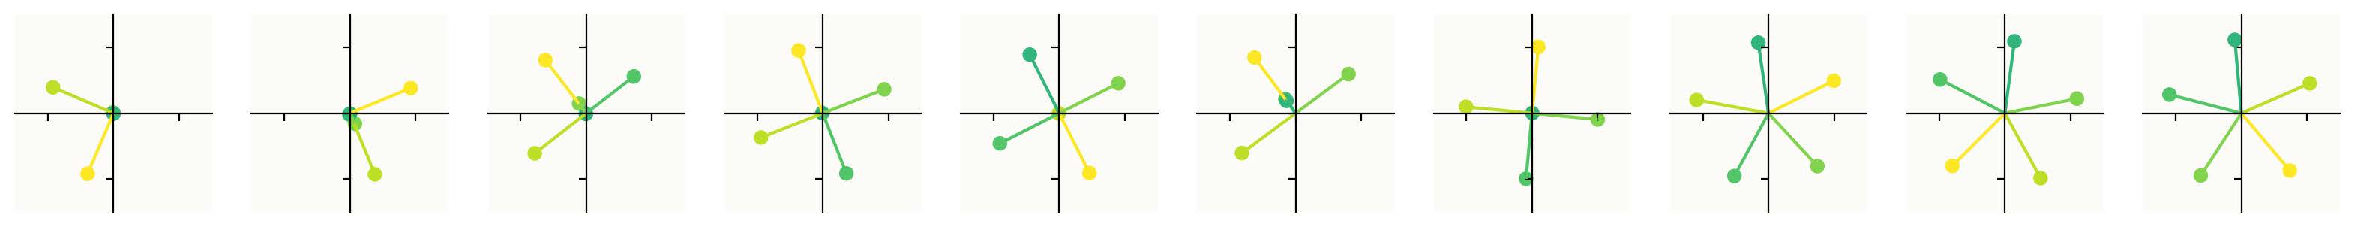
\includegraphics[width=\textwidth]{tmlr_paper/images/intro_diagram.pdf}\\
  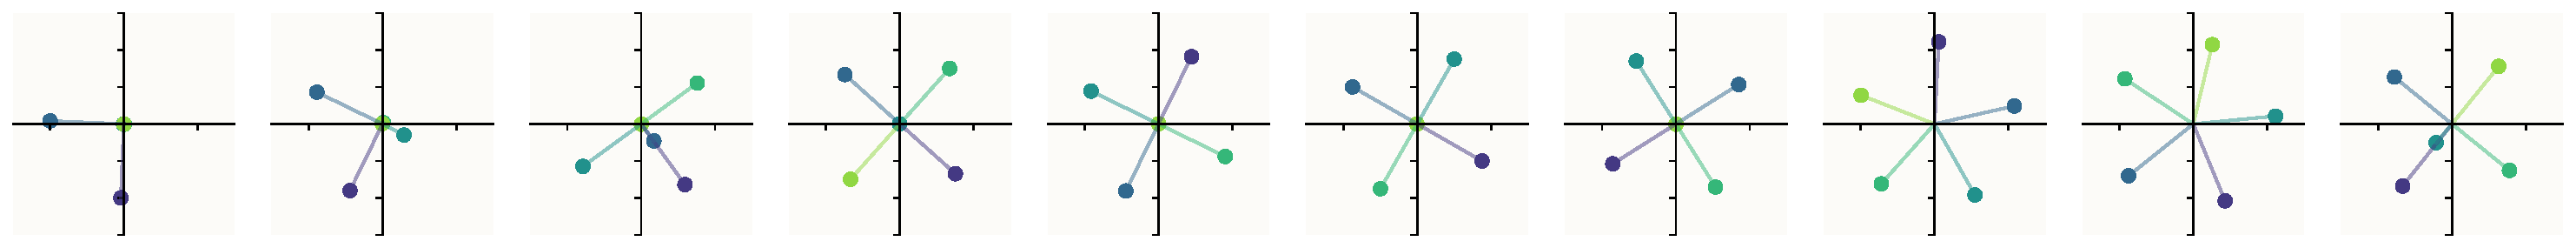
\includegraphics[width=\textwidth]{tmlr_paper/images/jerge_intro_diagram.pdf}
  \caption{Visualization of superposition. Each feature's learned embedding is plotted as a vector in a non-privileged, two-dimensional
  coordinate system derived from the model's weight matrix. The top panel displays results from code provided by the authors of the
  original paper \citep{elhage2022}; the bottom panel shows the results from our replication. Further replication results can be found in
  our repository. \url{https://github.com/mmjerge/superposition_replication}}
  \label{fig:superposition}
\end{figure}

Each panel shows feature embeddings as vectors in 2D space, derived from columns of the learned weight matrix $W$. When superposition occurs, we observe more than $m=2$ features represented as distinct directions, often arranged with approximately equal angular spacing (e.g., pentagon or hexagon patterns for 5--6 features). The top row shows results from the original authors' code; the bottom row shows our independent implementation.

Our replicated results closely match the original findings. Without ReLU (the linear model), features collapse or align with the two available dimensions---no superposition occurs because interference cannot be managed. In contrast, with ReLU, features arrange themselves in geometric patterns (pentagons, hexagons) that maximize angular separation, representing more features than dimensions. This is superposition in action.

We also observe the predicted effects of sparsity and importance. As sparsity increases (features less frequently active), models represent more features in superposition because interference costs decrease. Meanwhile, high-importance features tend to occupy dedicated dimensions, while lower-importance features are more likely to be superposed.

These results confirm the core finding: ReLU-based autoencoders develop superposition as a strategy for representing more features than dimensions, with the degree of superposition governed by feature sparsity and importance.